\documentclass[12pt,oneside,a4paper,article]{abntex2}
\usepackage[utf8]{inputenc} % Codificação do documento
\usepackage{lmodern}
\usepackage[brazil]{babel}  % Idioma do documento
\usepackage{graphicx}       % Inclusão de gráficos
\usepackage{tabularx}       % Tabelas avançadas
\usepackage{amsmath}        % Melhorias em matemática
\usepackage{lipsum}         % Geração de texto dummy
\usepackage{authblk}
\usepackage{parskip}
\usepackage{pdfpages}

% Configurações específicas do abntex2
% Aqui você pode adicionar configurações específicas, como redefinições de comandos
% ou adições de novos pacotes que são essenciais para o seu documento.

% Carrega o pacote abntex2cite para citações
\usepackage[alf]{abntex2cite} % ou use [num] para citações numéricas

\usepackage[left=3cm,right=2.5cm,top=3cm,bottom=2cm]{geometry} % Margens
\usepackage{setspace}       % Espaçamento entre linhas
% %\usepackage{natbib}      % Formatação de bibliografia

% Informações de título
\title{\textbf{Documento Mangaba's Kitchen}}
\author{Evellyn Costa \thanks{evellyn.pedroso@ucsal.edu.br}}
\author{Guilherme Vieira \thanks{guilhermenovais.vieira@ucsal.edu.br}}
\author{Henrique Silva \thanks{henrique.souza@ucsal.edu.br}}
\author[1]{Lucas Santos \thanks{lucassantos.garrido@ucsal.edu.br}}
\author[1]{Maria Luisa \thanks{marialuisacarvalho.silva@ucsal.edu.br}}
\author[1]{Victor Dantas \thanks{victor.dantas@ucsal.edu.br} }
\author[1]{Vinicius Kauan \thanks{viniciuskauan.cruz@ucsal.edu.br} }
\author[1*]{Elton Figueiredo \thanks{elton.figueiredo@pro.ucsal.br}}
\affil{
    Engenharia de Software \par
    Escola de Tecnologias \par
    Universidade Católica do Salvador (UCSAL) \par
    Av. Prof. Pinto de Aguiar, 2589 Pituaçu, CEP: 41740-090 \par
    Salvador/BA, Brasil
}
% \affil[1]{\textit {\{evellyn.pedroso,henrique.souza,lucassantos.garrido,guilhermenovais.vieira\}@ucsal.edu.br}}
% affil[1]{\textit {\{marialuisacarvalho.silva,victor.dantas,viniciuskauan.cruz\}@ucsal.edu.br}}
% \affil[1*]{\textit {\{elton.figueiredo\}@pro.ucsal.edu.br}}

\date{Setembro 2024}

\newpage

\ifthenelse{\equal{\ABNTEXisarticle}{true}}{%
\renewcommand{\maketitlehookb}{}
}{}

% Configurações de aparência do PDF final
% \usepackage{hyperref} % para inserir links
\hypersetup{
    colorlinks=false,       % false: boxed links; true: colored links
    pdfborder={0 0 0},      % remove as bordas ao redor dos links
}

\newpage
\renewcommand*{\Authsep}{, }
\renewcommand*{\Authand}{, }
\renewcommand*{\Authands}{, }
\renewcommand*{\Affilfont}{\normalsize\normalfont}
\renewcommand*{\Authfont}{\bfseries}    % make author names boldface    
\setlength{\affilsep}{2em}   % set the space between author and affiliation

\newsavebox\affbox



\newpage


\begin{document}

    \begin{center}
        
\includegraphics[width=0.3\textwidth]{imagens-template/ucsal_logo.png} 
    \end{center}
    {\let\newpage\relax\maketitle}
    
    \begin{center}
        \textbf{Cliente: Mateus de Jesus Rocha}
    \end{center}
    
    \newpage
    \begin{resumoumacoluna}
    \hspace{4.5mm}
O projeto de informatização do Mangaba's Kitchen visa desenvolver um sistema informatizado para o restaurante Mangaba Kitchen, com o objetivo de otimizar o controle de pedidos e estimativas de entrega. A iniciativa busca resolver problemas relacionados à falta de precisão nas previsões de tempo e à dificuldade em gerenciar o fluxo de pedidos, impactando negativamente a experiência dos clientes e a eficiência operacional do restaurante. A solução proposta inclui a criação de um sistema integrado que melhora a comunicação entre garçons e cozinha, oferecendo estimativas de tempo mais precisas e um controle mais eficiente dos pedidos.
O sistema contará com três interfaces principais: uma para o gerente, que gerencia o cadastro de funcionários, pratos e formas de pagamento, além de gerar relatórios de comissão e faturamento; uma para os garçons, que permitirá o gerenciamento de mesas, adição de pedidos e visualização das estimativas de entrega; e uma para os cozinheiros, que possibilitará o gerenciamento dos pedidos em preparação, a visualização das receitas e o controle do tempo de preparo. Cada interface será projetada para atender às necessidades específicas dos usuários e garantir uma operação mais organizada.
Além das funcionalidades principais, como o controle de pedidos e estimativas de tempo, o sistema incluirá recursos de segurança, como logins individuais para os funcionários, e relatórios detalhados para melhorar a eficiência operacional. A informatização do pagamento servirá apenas para controle, sem transações financeiras diretas. Com essas melhorias, o projeto visa não apenas reduzir erros e atrasos, mas também proporcionar uma experiência mais satisfatória para os clientes e uma gestão interna mais eficiente.
    \vspace{\onelineskip}
     
    \noindent
    \textbf{Palavras-chaves}: Scrum, Kanban, Automação, Gestão, Escalabilidade, Usabilidade.
    \end{resumoumacoluna}
    
    \textual
    
    \vspace{12mm}
    
    \section{Introdução}                         
        \hspace{4.5mm}
O Mangaba Kitchen é um restaurante que se destaca por seu cardápio variado, com refeições completas durante o almoço e especialidades em pizza e hambúrgueres à noite. Com o crescimento das operações e a complexidade crescente no gerenciamento de pedidos, o restaurante identificou a necessidade de uma solução tecnológica para melhorar a eficiência e a precisão no atendimento. Atualmente, a coordenação entre os garçons e a cozinha enfrenta desafios que podem levar a atrasos e erros nos pedidos, impactando diretamente a satisfação dos clientes.             
    \vspace{12mm}                                
    
    \newpage                                     
    \section{Definição do Cliente}               
        \hspace{4.5mm}
O restaurante Mangaba's Kitchen, que oferece almoço à tarde e, à noite, pizza e hambúrgueres, está em processo de informatização de seu sistema de pedidos. O objetivo principal, segundo o cliente, é otimizar o controle sobre a estimativa de entrega dos pratos e melhorar a gestão dos pedidos. O restaurante deseja implantar um sistema com login e senha individual para cada funcionário, inclusive cozinheiros, com renovação obrigatória da senha a cada três meses. Além disso, o app precisa se integrar aos pedidos feitos por delivery e fornecer uma interface para os garçons registrarem os pedidos feitos localmente, facilitando a comunicação entre o salão e a cozinha.
\par
A funcionalidade principal para o cozinheiro/chef, considerando o que o cliente falou, é a tela que permite adicionar os pedidos à "fila de espera", ajustando automaticamente o tempo estimado de preparo. O cozinheiro também pode ajustar manualmente o tempo de preparo dos pratos conforme necessário. Para auxiliar na execução, cada prato na fila deve exibir a receita correspondente. Para os garçons, a interface possibilitará a adição dos pedidos de cada mesa, com um sistema que calcula o valor total conforme os itens são inseridos. No final do dia, o sistema poderá gerar relatórios de faturamento, separando por mesa e por garçom.
\par
Além disso, foi reforçado que o sistema precisa incluir funcionalidades para gerar relatórios de comissão dos garçons e aplicar descontos financeiros em caso de erros na preparação dos pratos, descontando o valor dos responsáveis (cozinha ou garçom, dependendo da falha). O sistema também deve permitir a informatização dos métodos de pagamento, registrando se o pagamento foi feito à vista, por crédito ou débito. Embora haja uma integração com o delivery, o sistema não é um serviço de entrega terceirizado como o iFood, sendo exclusivo para uso interno do restaurante.              
    \vspace{12mm}                                
    
    \newpage                                        
    \section{Entrevista com o Cliente}              
        \hspace{4.5mm}
A entrevista com os clientes do restaurante Mangaba's Kitchen foi conduzida para esclarecer alguns pontos que estavam pendentes no projeto de automação do sistema de atendimento. O foco da conversa foi entender melhor as expectativas dos proprietários em relação à padronização do atendimento e à redução de prejuízos. A proposta da empresa foi desenvolver um sistema que utilizasse tablets, tanto para os funcionários quanto para os clientes, oferecendo funcionalidades que incluíssem desde a visualização dos pratos até a identificação dos responsáveis pela preparação. A ideia central era criar uma solução que atendesse às demandas do restaurante de forma eficiente e ágil, garantindo um melhor controle dos processos internos e uma experiência mais organizada para os clientes.
\par
Para os garçons, o sistema incluirá uma tela de cadastro, associando cada funcionário ao nome e função. Além disso, será possível vincular cada garçom às mesas que ele atende, registrando o valor dos pratos vendidos e as especificações dos pedidos feitos pelos clientes. No final de cada dia, o sistema gerará um resumo com as informações dos pratos preparados e as vendas realizadas por cada garçom. Já para os cozinheiros, a proposta é semelhante, com o sistema registrando os pratos preparados, o cozinheiro responsável por cada pedido e um relatório diário de desempenho. Essa automação permitirá um maior controle da produtividade e uma melhor coordenação entre o salão e a cozinha.
\par
Além das funcionalidades voltadas para a equipe, o sistema incluirá tablets em cada mesa, permitindo que os clientes visualizem o cardápio, valores dos pratos e especificações, assim como o nome do garçom responsável pelo atendimento. Na cozinha, uma televisão exibirá o nome dos pratos, o tempo estimado de preparo e as especificações dos pedidos, facilitando o trabalho dos cozinheiros e garantindo uma entrega mais precisa e dentro do prazo. Embora os clientes não tenham especificado detalhes de layout, eles demonstraram satisfação com a logo criada pela equipe de design e prometeram fornecer referências para ajudar na criação de uma interface que atenda melhor às suas preferências estéticas.                
    \vspace{12mm}                                   
    
    \newpage                                
    \section{Problema}                      
        \hspace{4.5mm}
\subsection{Introdução} O restaurante cliente enfrenta desafios críticos no controle da entrega de pratos e no gerenciamento dos pedidos dos clientes. A falta de um sistema eficiente para estimar com precisão o tempo de entrega e organizar adequadamente os pedidos compromete a experiência dos clientes, prejudica a eficiência operacional e afeta a precisão do serviço. Esses problemas geram dificuldades na comunicação do tempo de espera, aumento da frustração dos clientes e falta de controle sobre o fluxo de trabalho da cozinha, impactando negativamente tanto a satisfação do cliente quanto a eficácia do restaurante.

\subsection{Descrição do Problema} O problema pode ser subdividido em dois aspectos principais:

\textbf{Estimativa de Tempo de Entrega} Atualmente, o restaurante não possui um sistema eficiente para prever o tempo necessário para preparar e entregar os pratos aos clientes. Isso resulta em: 
\begin{itemize} 
    \item Dificuldade em informar o tempo exato de entrega ao cliente; 
    \item Incerteza em relação ao prazo, causando frustração para os clientes; 
    \item Falta de controle sobre o fluxo de trabalho da cozinha, o que pode gerar atrasos ou confusão na preparação dos pratos. 
\end{itemize}

\textbf{Controle dos Pedidos} O sistema de controle de pedidos também apresenta dificuldades em: 
\begin{itemize} 
    \item Monitorar os pedidos em andamento, identificando quais estão prontos e quais ainda precisam ser preparados; 
    \item Gerenciar o fluxo de trabalho de maneira eficiente para otimizar a produção e evitar acúmulo de pedidos; 
    \item Manter um histórico preciso dos pedidos para gerar relatórios de desempenho e melhorar a operação futura. 
\end{itemize}

\textbf{Impacto do Problema} Esses problemas resultam em uma série de desafios para o restaurante, incluindo: 
\begin{itemize} 
    \item Aumento da insatisfação dos clientes devido à demora e à falta de comunicação precisa sobre os tempos de entrega; 
    \item Ineficiência operacional que pode resultar em desperdício de tempo e recursos; 
    \item Dificuldade em melhorar os processos internos devido à falta de dados precisos sobre o desempenho dos pedidos. 
\end{itemize}

\textbf{Proposta de Solução} Para mitigar os problemas identificados, sugerimos a implementação de um sistema que ofereça: 
\begin{itemize} 
    \item Estimativas precisas e em tempo real do tempo de entrega de cada prato; 
    \item Um painel de controle que permite ao restaurante visualizar todos os pedidos em andamento, juntamente com seu status e prazo estimado de conclusão; 
    \item Relatórios de desempenho que permitam analisar tempos de preparo e entrega para melhorias contínuas. 
\end{itemize}

\subsection{Conclusão} A implementação de um sistema integrado para controle de estimativa de tempo e pedidos ajudará o restaurante a melhorar sua eficiência, reduzir atrasos e oferecer uma experiência mais satisfatória aos seus clientes.          
    \vspace{12mm}                           
    
    \newpage                                
    \section{Objetivo}                      
        \hspace{4.5mm}
O principal objetivo do sistema para o Mangaba Kitchen é otimizar a operação do restaurante, melhorando o controle sobre as estimativas de entrega dos pratos e o gerenciamento dos pedidos. Com a crescente complexidade na coordenação entre a equipe de garçons e a cozinha, é fundamental estabelecer um sistema eficiente que não só simplifique a comunicação interna, mas também eleve a qualidade do serviço prestado aos clientes. A implementação de um sistema informatizado visa resolver os problemas atuais e promover uma operação mais organizada e ágil.
\par
Para atingir esse objetivo, o sistema será projetado com várias funcionalidades específicas. Primeiramente, será criado um controle de acesso para funcionários, com logins e senhas individuais, assegurando a segurança e a responsabilidade na operação. Além disso, uma interface para a cozinha permitirá a gestão estruturada dos pedidos, incluindo a capacidade de adicionar pratos à “fila de espera” e ajustar o tempo de preparo conforme necessário. Os cozinheiros também terão acesso às receitas detalhadas dos pratos, o que ajudará a garantir a precisão na preparação e a reduzir erros. Paralelamente, os garçons utilizarão uma interface dedicada para registrar pedidos diretamente, o que facilitará a comunicação do salão e da cozinha.
\par
Além dos aspectos operacionais, o sistema também abordará questões relacionadas à transparência e responsabilização. Será implementado um mecanismo para gerar relatórios detalhados sobre a comissão dos garçons e registrar erros na preparação dos pratos, aplicando desconto financeiro em caso de falhas. Também será criado um sistema de crítica para garantir que os garçons verifiquem restrições alimentares dos clientes, com penalizações em caso de negligência. Esses objetivos visam promover um ambiente de trabalho mais eficiente, seguro e orientado à qualidade, resultando em um melhor atendimento ao cliente e uma operação interna mais fluida e bem organizada.          
    \vspace{12mm}                           
    
    \newpage                                            
    \section {Requisitos Funcionais e Não-Funcionais}   
        \hspace{4.5mm}
\subsection{Introdução}
Este documento de requisitos descreve as funcionalidades e as características do sistema a ser desenvolvido para um restaurante, visando solucionar os problemas de controle de estimativa de entrega dos pratos e gerenciamento de pedidos. O objetivo é melhorar a eficiência operacional e a satisfação dos clientes.

\subsection{Escopo}
O sistema será desenvolvido para gerenciar o fluxo de pedidos, estimar o tempo de entrega e fornecer relatórios que auxiliem no controle de desempenho do Mangaba's Kitchen, sendo unica e exclusivamente direcionado ao mesmo. Ele será implantado para o ambiente de cozinha quanto para a equipe de salão do restaurante.

\subsection{Requisitos Funcionais}
Os requisitos funcionais especificam as funcionalidades que o sistema deve proporcionar para atender efetivamente às necessidades do cliente e resolver os problemas identificados. Esses requisitos detalham as operações e capacidades que o sistema deve possuir para garantir que todas as operações do restaurante sejam gerenciadas de forma eficiente e eficaz.

\begin{itemize}
    \item \textbf{Estimativa de Tempo de Entrega:} O sistema deve calcular o tempo estimado para a preparação e entrega de cada prato e exibi-lo ao cliente no momento da realização do pedido.
    
    \item \textbf{Controle de Pedidos:} O sistema deve permitir que a equipe do restaurante acompanhe o status de cada pedido, desde o momento em que ele é recebido até sua finalização (preparado e entregue).
    
    \item \textbf{Atualização do Status dos Pedidos:} O sistema deve permitir que a cozinha atualize o status dos pedidos, informando quando o prato está em preparação e quando está pronto para ser entregue.
    
    \item \textbf{Histórico de Pedidos:} O sistema deve armazenar um histórico de todos os pedidos realizados, permitindo a geração de relatórios sobre o tempo de preparo e entrega para análise posterior.
    
    \item \textbf{Notificações para os Garçons:} O sistema deve enviar notificações automáticas aos garçons informando sobre o status dos pedidos ativos na interface daquele garçom específico, especialmente quando o prato estiver pronto para ser entregue.
\end{itemize}

\subsection{Requisitos Não Funcionais}
Os requisitos não funcionais descrevem as características e qualidades que o sistema deve ter para garantir sua eficácia e boa operação. Eles incluem aspectos como desempenho, segurança, usabilidade e manutenção. No contexto do projeto para o Mangaba Kitchen, esses requisitos garantem que o sistema não só funcione corretamente, mas também atenda a padrões elevados de qualidade e eficiência.

\begin{itemize}
    \item \textbf{Performance:} O sistema deve calcular e exibir o tempo estimado de entrega em tempo real, sem atrasos significativos, para garantir a precisão das informações fornecidas aos clientes.
    
    \item \textbf{Confiabilidade:} O sistema deve ser altamente confiável, garantindo que os pedidos não sejam perdidos ou processados incorretamente, independentemente da quantidade de pedidos sendo feitos simultaneamente.
    
    \item \textbf{Usabilidade:} O sistema deve ser fácil de usar tanto para os funcionários do restaurante quanto para os clientes, com uma interface simples e intuitiva.
    
    \item \textbf{Escalabilidade:} O sistema deve ser capaz de lidar com um aumento no número de pedidos e pratos sem comprometer o desempenho ou a precisão das estimativas de tempo.
    
    \item \textbf{Segurança:} O sistema deve proteger os dados dos funcionários entre si, clientes e dos pedidos contra acessos não autorizados, garantindo a privacidade e a segurança das informações.
\end{itemize}

\subsection{Conclusão}
Este documento de requisitos especifica as funcionalidades e características que o sistema proposto deve apresentar para melhorar o controle de estimativa de entrega e o gerenciamento de pedidos no restaurante. A implementação desse sistema contribuirá para otimizar a operação interna e proporcionar uma melhor experiência aos clientes.                    
    \vspace{12mm}                                       
    
    \newpage                            %%%%%%%
    \section{Telas do Figma}            %%%%%%%     Definição e conceito de cada tela
        \listoffigures
\newpage

\begin{center}
    \subsection{Telas do Gerente}
    \begin{figure}[!htp]
        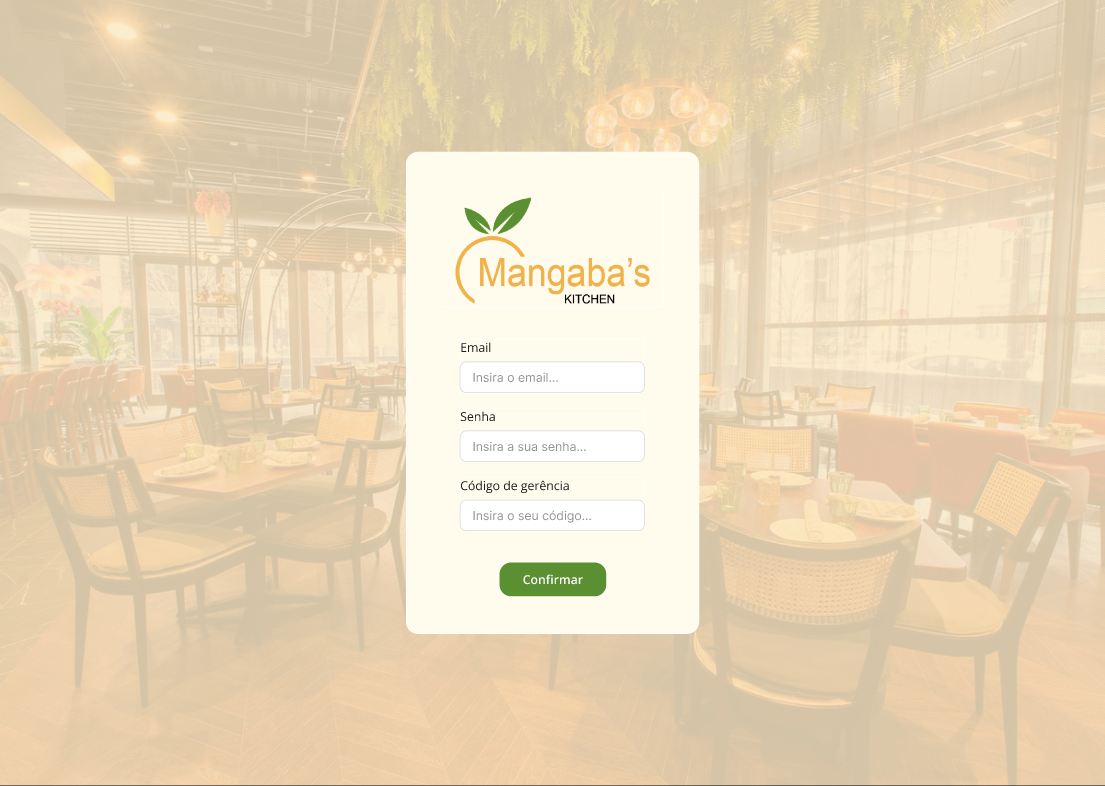
\includegraphics[width=1\textwidth]{imagens-template/Layout_Gerente_2638.png} 
        \caption{Tela de login do gerente.}
    \end{figure}
    \newpage
    \begin{figure}[!htp]
        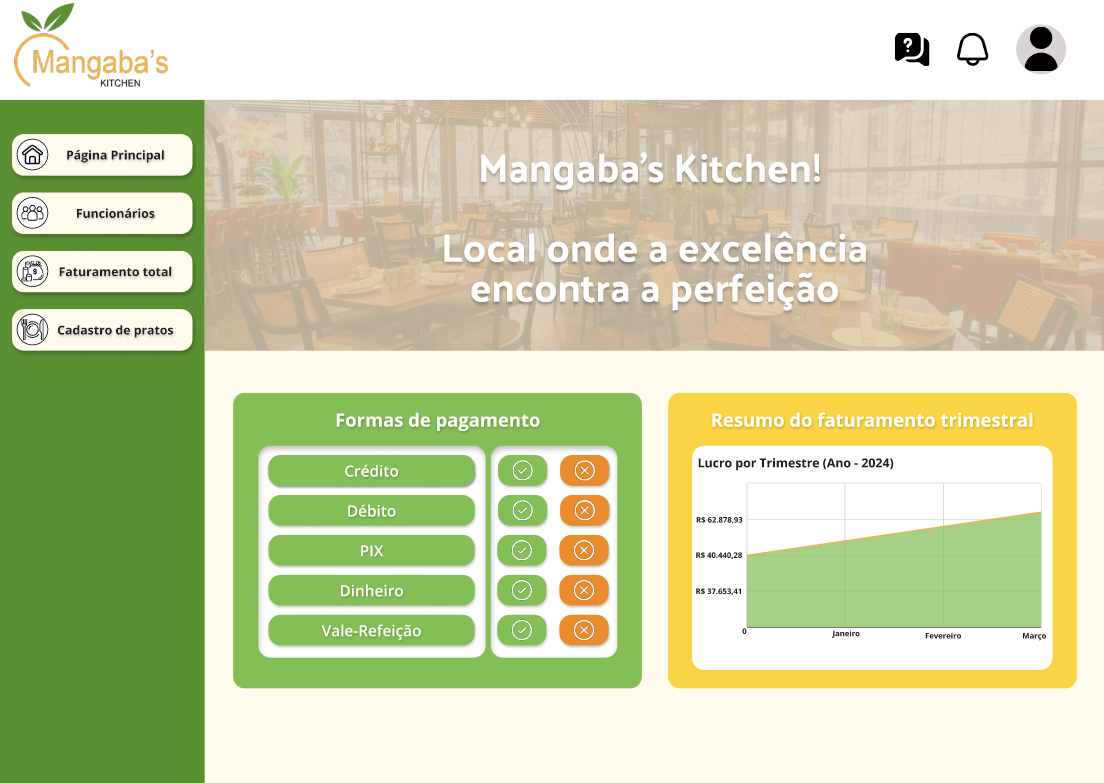
\includegraphics[width=1\textwidth]{imagens-template/Layout_Gerente_2700.png} 
        \caption{Painel inicial do gerente, com gerenciamento dos meios de pagamento e um gráfico trimestral do faturamento do restaurante.}
    \end{figure}
    \newpage
    \begin{figure}[!htp]
        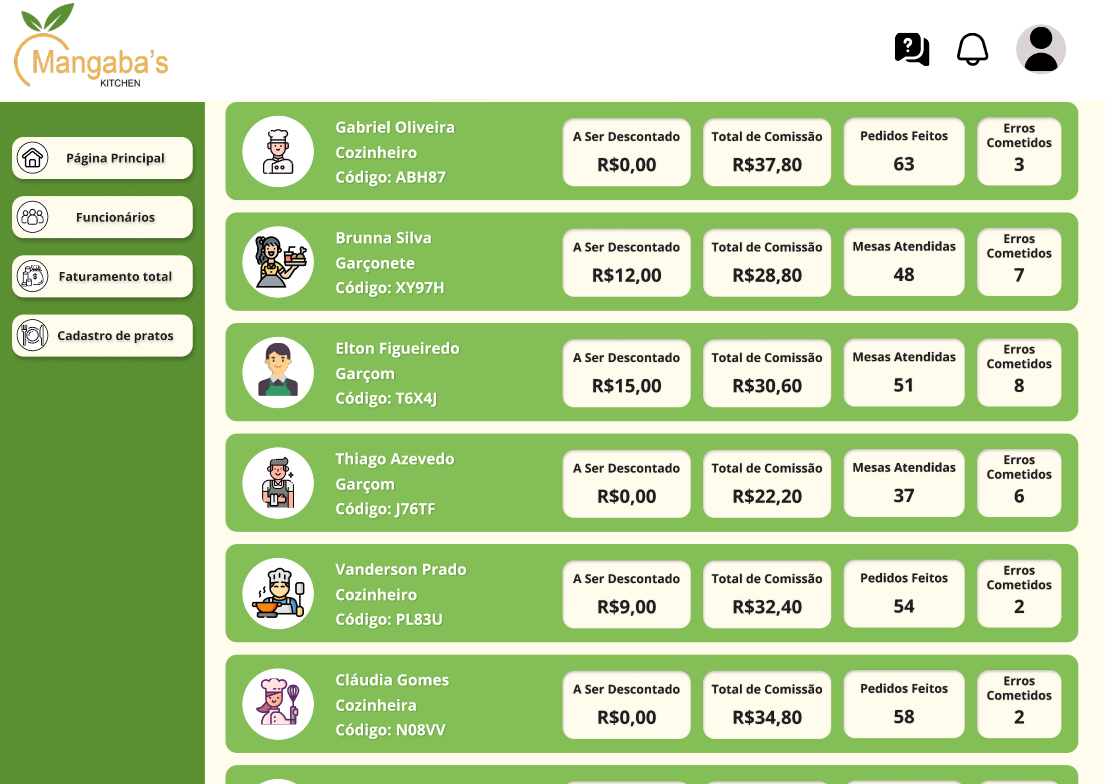
\includegraphics[width=1\textwidth]{imagens-template/Layout_Gerente_2659.png} 
        \caption{Painel de funcionários com as informações mais relevantes, como prejuízo causado e lucro gerado.}
    \end{figure}
    \newpage
    \begin{figure}[!htp]
        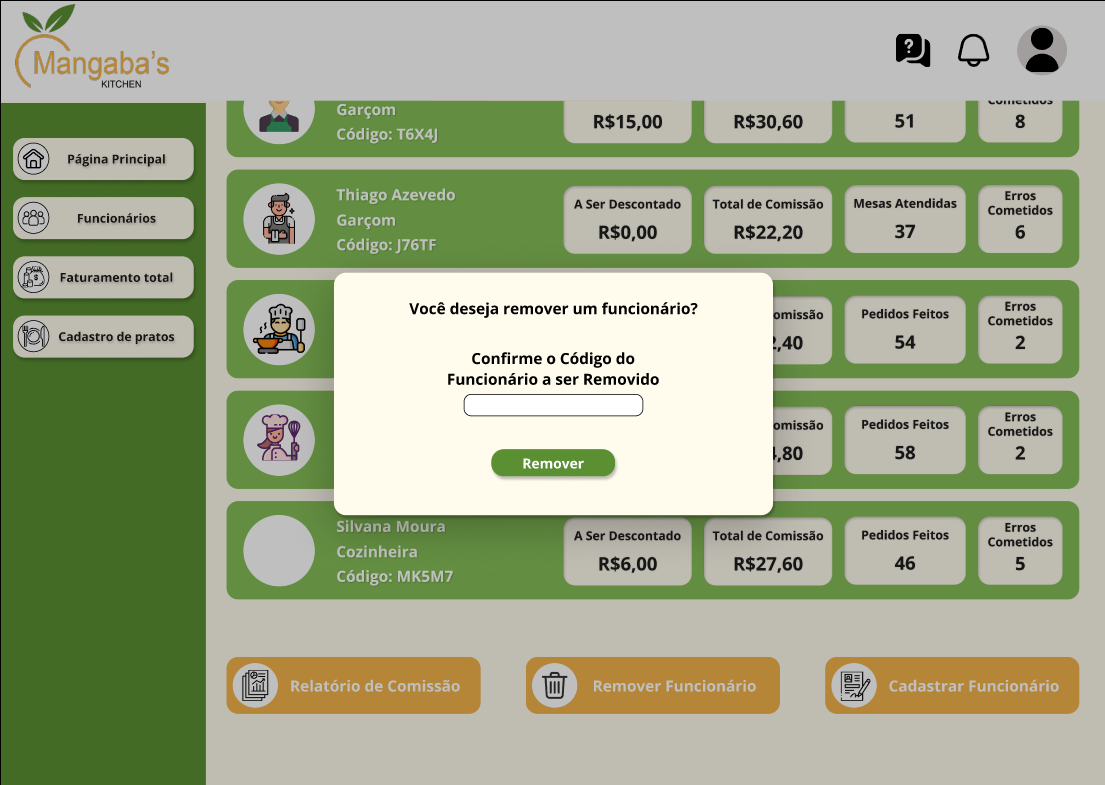
\includegraphics[width=1\textwidth]{imagens-template/Layout_Gerente_2657.png} 
        \caption{Pop-up de remoção de funcionário, pedindo o código como confirmação.}
    \end{figure}
    \newpage
    \begin{figure}[!htp]
        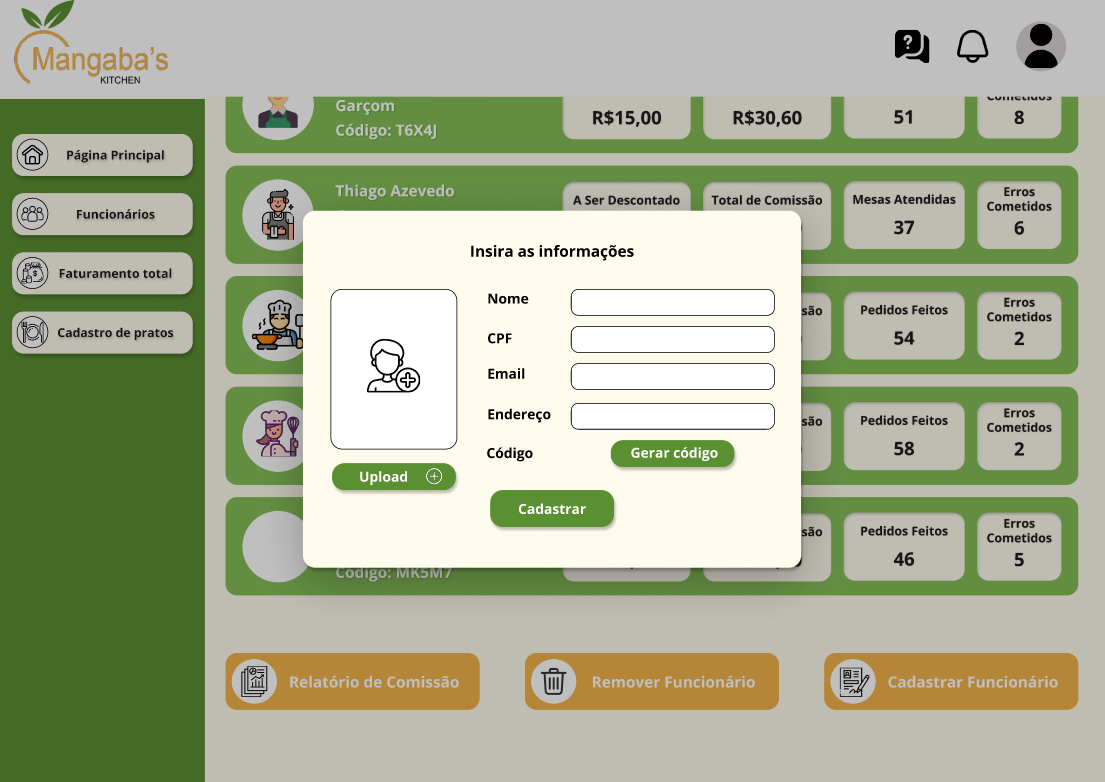
\includegraphics[width=1\textwidth]{imagens-template/Layout_Gerente_2655.png} 
        \caption{Pop-up de cadastro de funcionário, com os campos nome, cpf, email, endereço e um código gerado aleatóriamente, que se renova a cada 3 meses. Também há a opção do upload da foto do funcionário para melhor identificação.}
    \end{figure}
    \newpage
    \begin{figure}[!htp]
        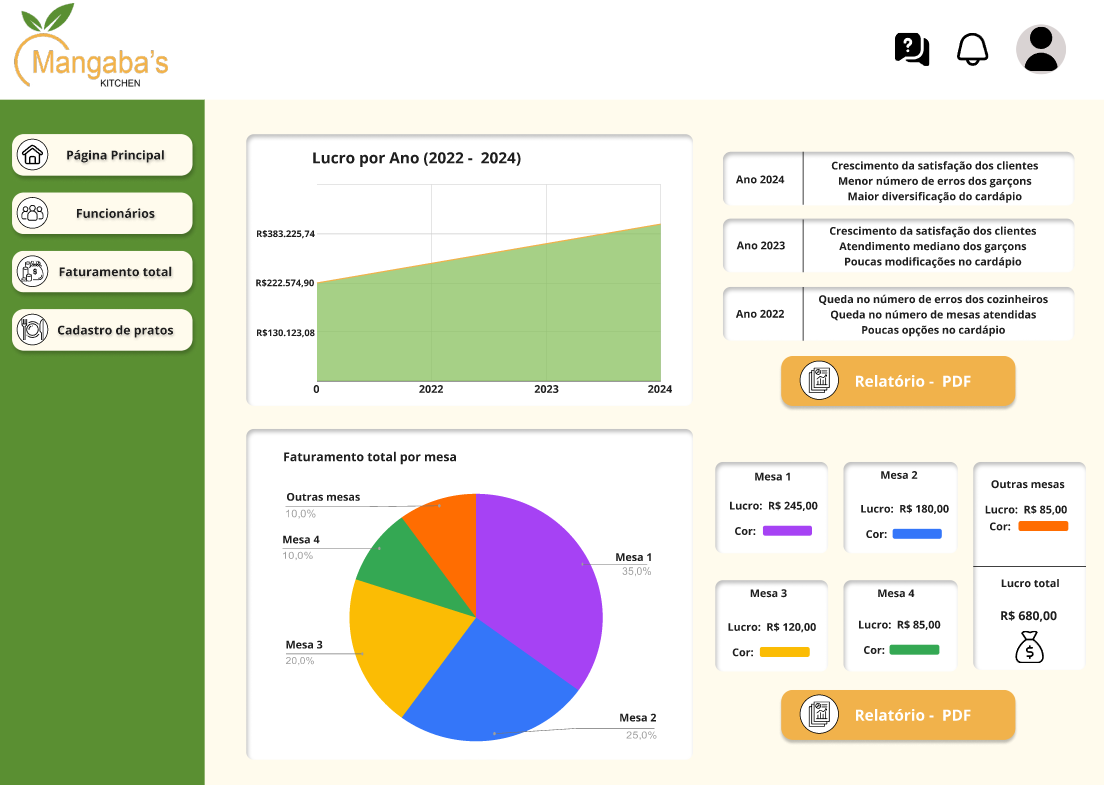
\includegraphics[width=1\textwidth]{imagens-template/Layout_Gerente_2653.png} 
        \caption{Tela de faturamento, com gráficos anuais e lucro por mesa, com uma definição construída pelo software e com opção para emissão de relatório.}
    \end{figure}
    \newpage
    \begin{figure}[!htp]
        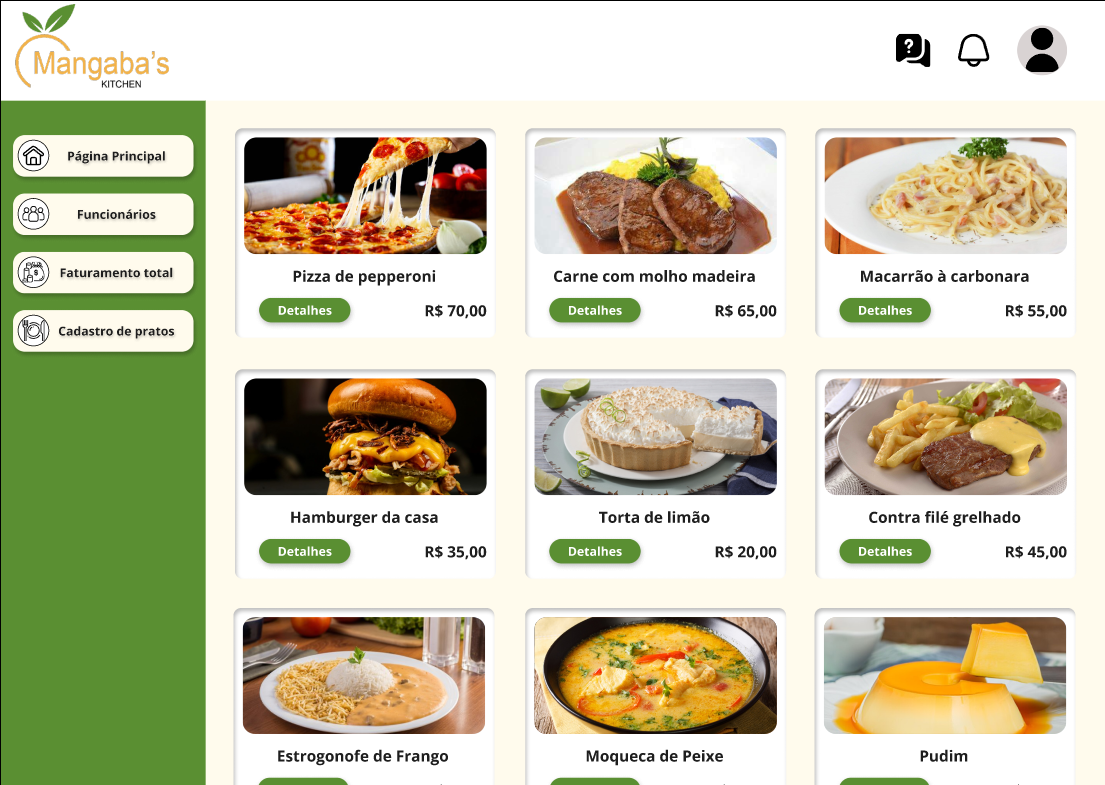
\includegraphics[width=1\textwidth]{imagens-template/Layout_Gerente_2651.png} 
        \caption{Painel de pratos cadastrados.}
    \end{figure}
    \newpage
    \begin{figure}[!htp]
        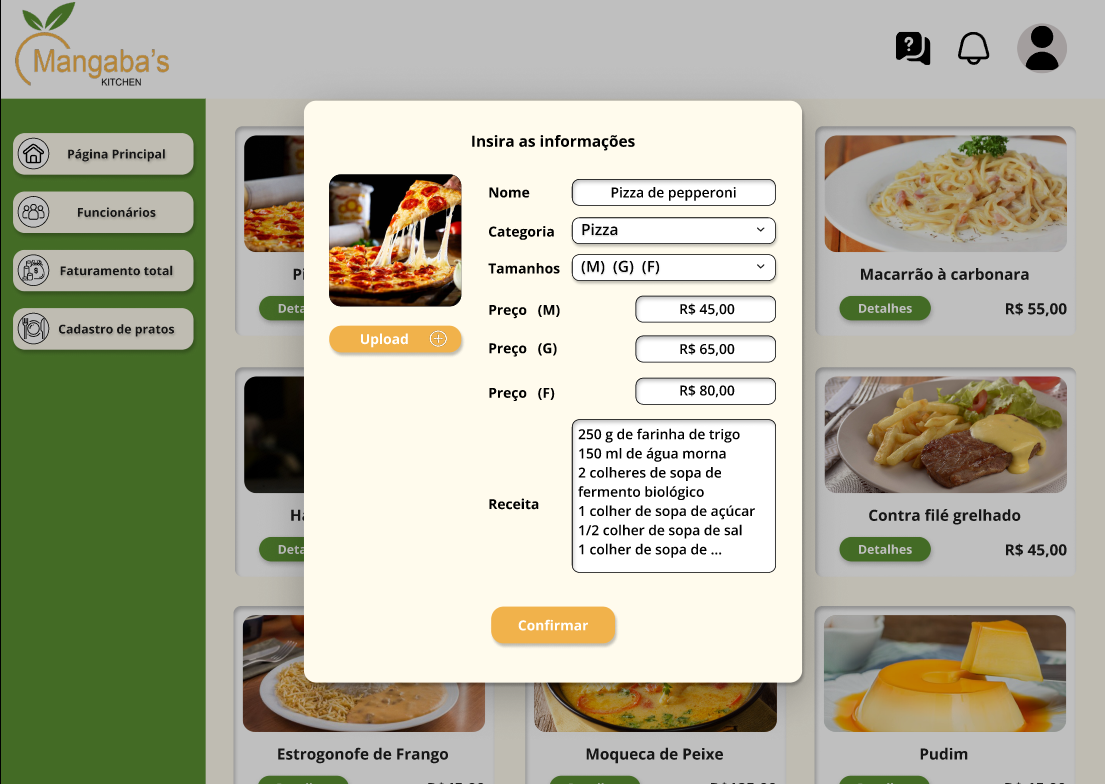
\includegraphics[width=1\textwidth]{imagens-template/Layout_Gerente_2649.png} 
        \caption{Pop-up de detalhes do prato, com possibilidade de alterar qualquer informação do prato. Se os campos ficarem em branco, o prato não será mostrado no painel.}
    \end{figure}
    \newpage
    \begin{figure}[!htp]
        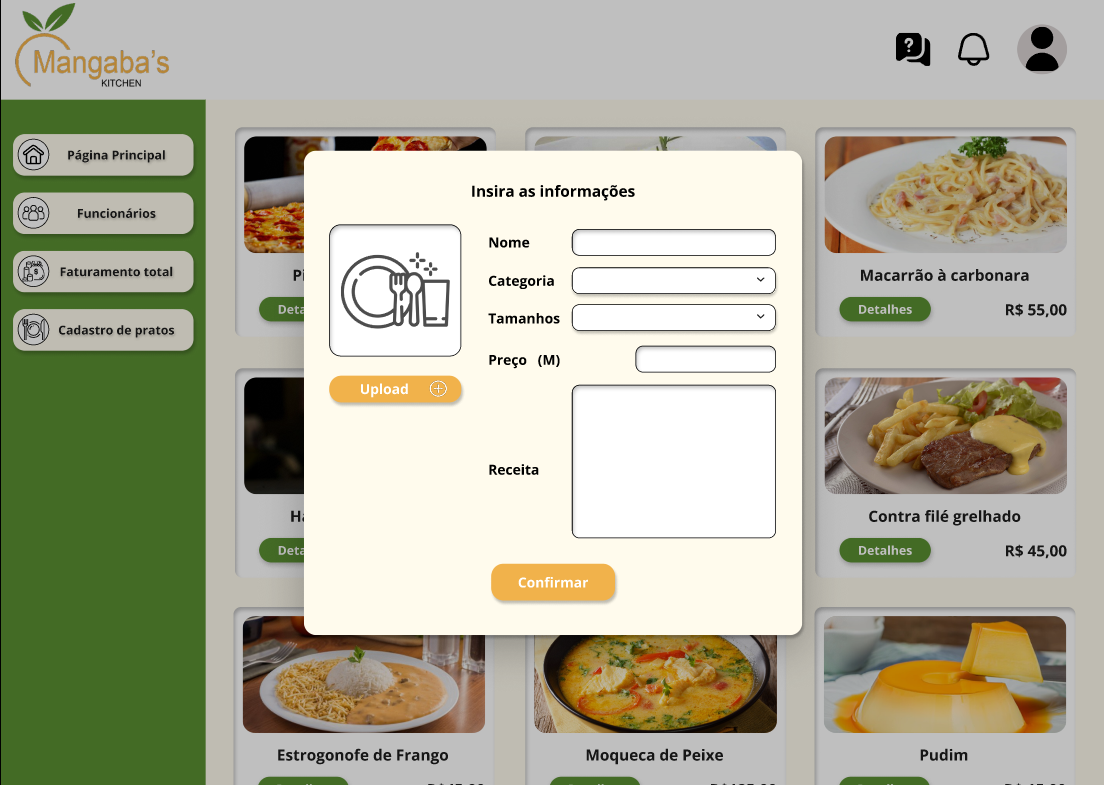
\includegraphics[width=1\textwidth]{imagens-template/Layout_Gerente_2647.png} 
        \caption{Pop-up de cadastro de prato, com opção para inserir uma imagem, selecionar o tamanho e o preço de cada tamanho disponível, além de um campo para inserir a receita. Se os campos ficarem em branco, o prato não será mostrado no painel.}
    \end{figure}
    \newpage
\end{center}

\newpage
\begin{center}
    \subsection{Telas do Garçom}
    \begin{figure}[!htp]
    \includegraphics[width=0.9\textwidth]{imagens-template/Layout_Garçom_2644.png} 
        \caption{Tela de login do funcionário.}
    \end{figure}
    \newpage
    \begin{figure}[!htp]
    \includegraphics[width=0.9\textwidth]{imagens-template/Layout_Garçom_2642.png} 
        \caption{Painel principal do garçom, com o controle de mesas ativas e inativas. Também a opção de consultar o histórico e cardápio.}
    \end{figure}
    \newpage
    \begin{figure}[!htp]
    \includegraphics[width=0.9\textwidth]{imagens-template/Layout_Garçom_2632.png} 
        \caption{Exemplo de uma mesa com pedido ativo. Há opções para inserir o modo de pagamento, nome do cliente, se é para levar ou não... Também é feita a soma de todos os itens no pedido e é mostrado para o garçom. Tem uma seção para verificar o status do pedido na cozinha e o tempo estimado para a finalização do prato. Mais abaixo são os itens do pedido e suas observações.}
    \end{figure}
    \newpage
    \begin{figure}[!htp]
    \includegraphics[width=0.9\textwidth]{imagens-template/Layout_Garçom_2629.png} 
        \caption{Pop-up para selecionar o meio de pagamento (Repare que a mesa está inativa).}
    \end{figure}
    \newpage
    \begin{figure}[!htp]
    \includegraphics[width=0.9\textwidth]{imagens-template/Layout_Garçom_2640.png} 
        \caption{Restante da página de mesa ativa, com o botão para adicionar mais itens ao pedido.}
    \end{figure}
    \newpage
    \begin{figure}[!htp]
    \includegraphics[width=0.9\textwidth]{imagens-template/Layout_Garçom_2634.png} 
        \caption{Consulta do cardápio que aparece quando o garçom precisa adicionar algum item no pedido. Os itens são separados em categorias.}
    \end{figure}
    \newpage
    \begin{figure}[!htp]
    \includegraphics[width=0.9\textwidth]{imagens-template/Layout_Garçom_2636.png} 
        \caption{Consulta individual do histórico de pedidos do garçom}
    \end{figure}
    \newpage
    \begin{figure}[!htp]
    \includegraphics[width=0.9\textwidth]{imagens-template/Layout_Garçom_2627.png} 
        \caption{Pop-up aberto ao clicar em "Detalhes", na aba de histórico. Aqui é mostrado ao usuário todas as informações sobre o pedido}
    \end{figure}
    \newpage
\end{center}

\begin{center}
    \subsection{Telas da Cozinha}
    \begin{figure}[!htp]
        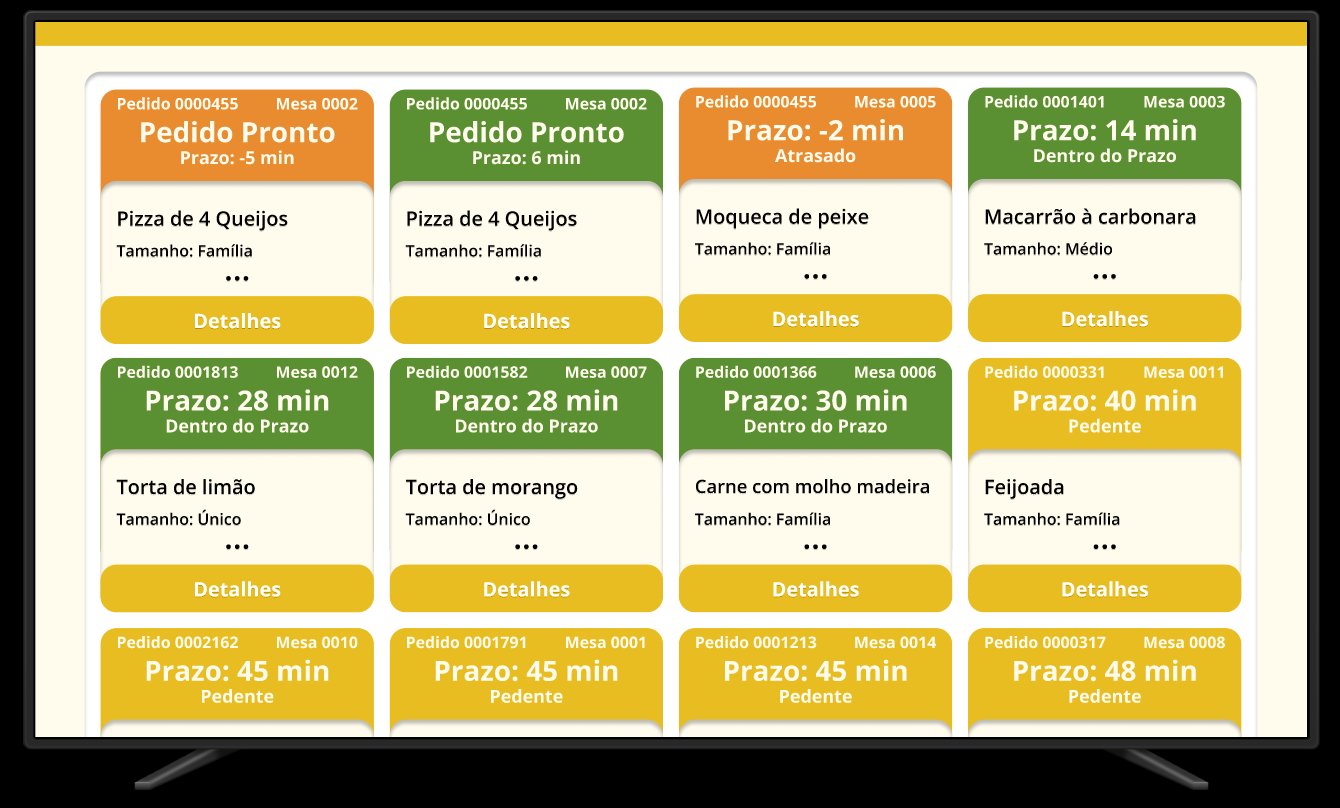
\includegraphics[width=1\textwidth]{imagens-template/Layout_Cozinha_2622.png}
        \caption{Painel da cozinha, mostrando o prazo para o pedido, se ele está pronto, o item daquele pedido, o número da mesa e o tamanho do item.}
    \end{figure}
    \newpage
    \begin{figure}[!htp]
        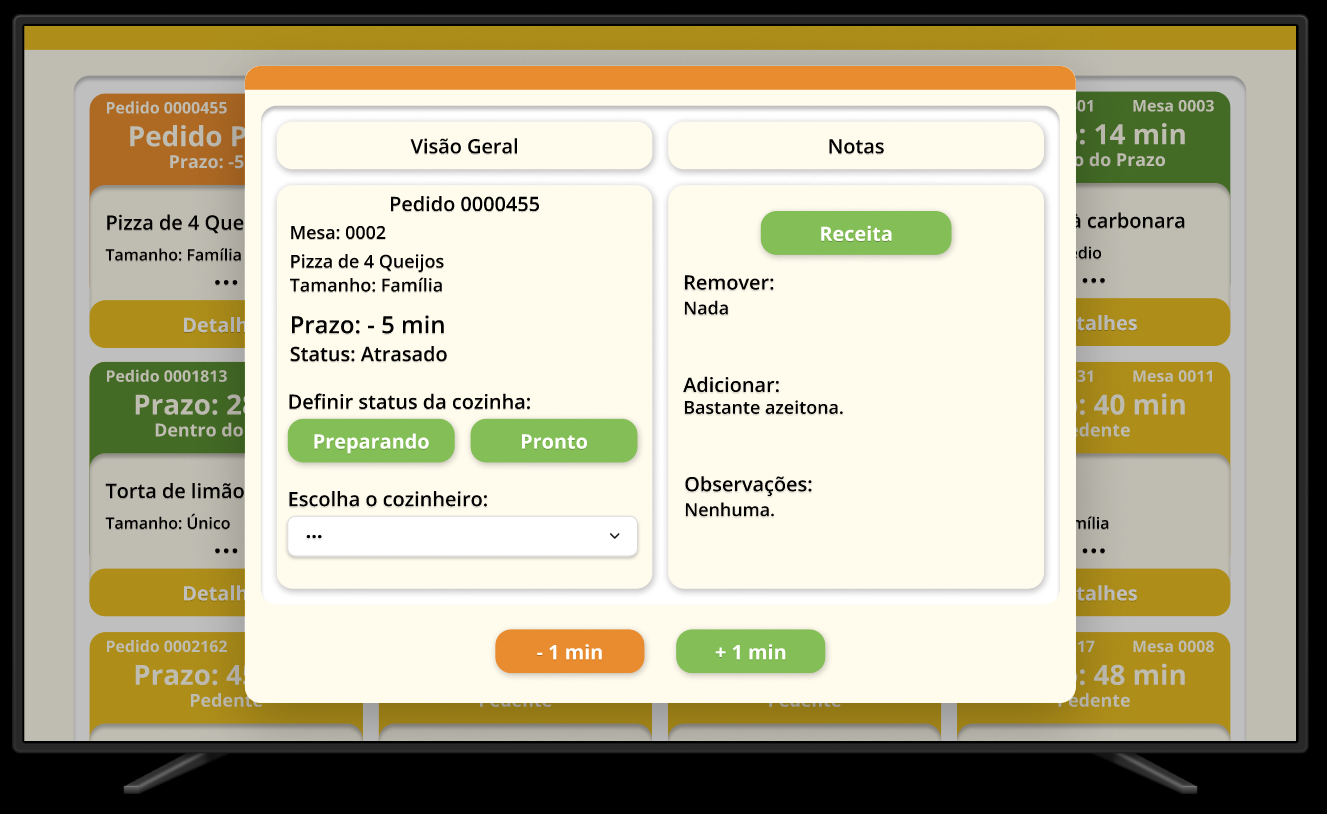
\includegraphics[width=1\textwidth]{imagens-template/Layout_Cozinha_2618.png}  
        \caption{Pop-ip de um pedido atrasado que foi aberto após o usuário clicar em "Detalhes" no painel principal. Aqui ele pode incrementar e decrementar o tempo, selecionar o cozinheiro responsável pelo pedido, e ver a receita do item.}
    \end{figure}
    \newpage
    \begin{figure}[!htp]
        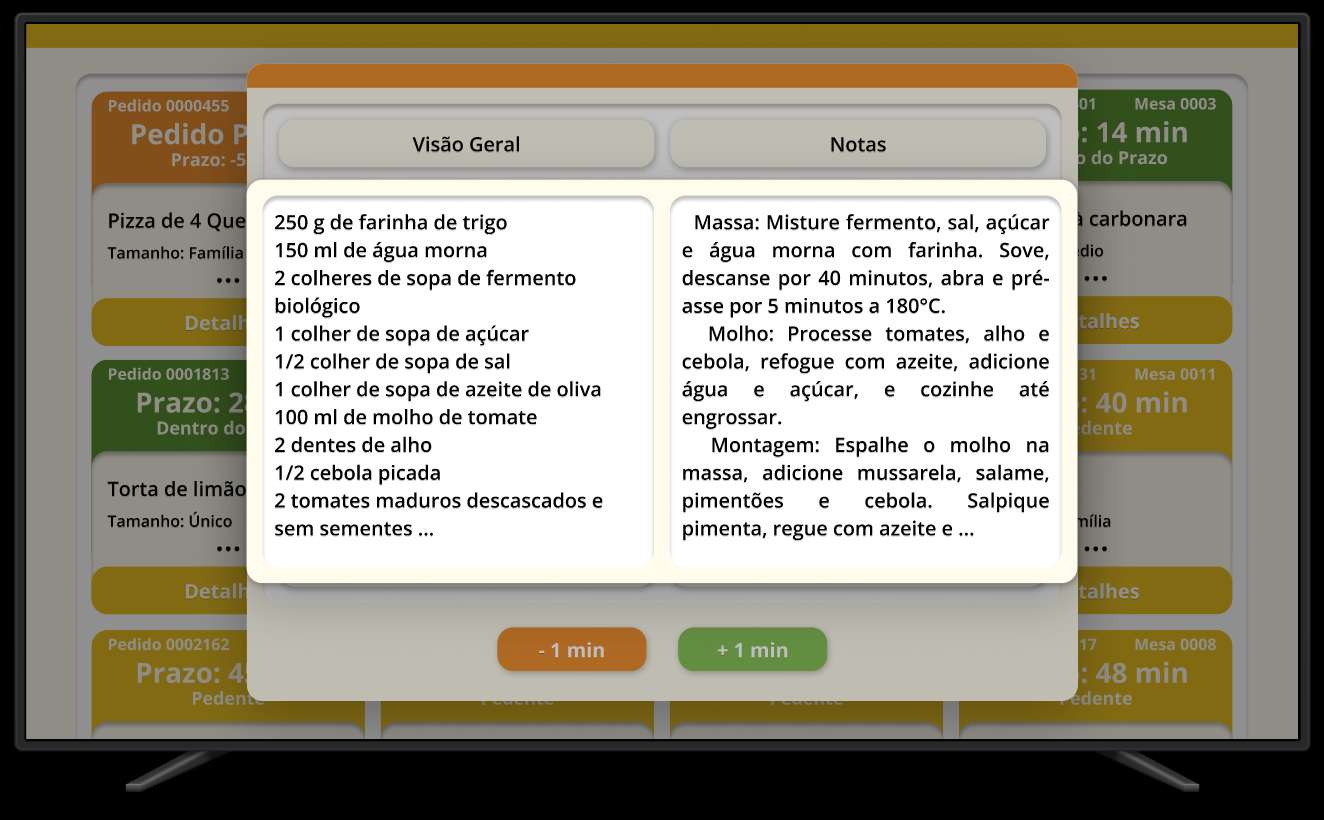
\includegraphics[width=1\textwidth]{imagens-template/Layout_Cozinha_2610.png} 
        \caption{Pop-up da receita do item}
    \end{figure} 
\end{center}         %%%%%%%
    \vspace{12mm}                       %%%%%%%
    
    \newpage
    \section{Análise de Viabilidade}
    \hspace{4.5mm}
\subsection {Viabilidade Organizacional e Operacional}
A viabilidade organizacional e operacional do projeto de informatização do Mangaba's Kitchen é altamente favorável, dada a forma como o sistema está alinhado com os objetivos estratégicos do restaurante e sua integração planejada nas operações diárias. O sistema, que inclui funcionalidades como controle de acesso e gerenciamento de pedidos, foi projetado para melhorar a eficiência e a comunicação interna entre gerentes, garçons e cozinheiros, facilitando o fluxo de trabalho e a coordenação entre as diferentes áreas. A escolha de dispositivos como iPads e uma TV touch, combinada com uma interface intuitiva, garante uma transição suave e a aceitação do sistema pela equipe. A abordagem metodológica Scrum permite um desenvolvimento iterativo, ajustando o sistema com base no feedback dos usuários e nas necessidades emergentes, o que assegura que o sistema continue a ser relevante e eficaz. Esse planejamento detalhado e a adaptação contínua asseguram que a implementação seja harmoniosa, sem interromper o fluxo de trabalho existente, e que a equipe possa rapidamente usufruir das melhorias proporcionadas pelo novo sistema.
\subsection {Viabilidade Econômica}
A viabilidade econômica do projeto de informatização do Mangaba's Kitchen está intrinsecamente ligada à análise das funcionalidades propostas e ao custo associado ao desenvolvimento do sistema. O sistema detalhado e bem delineado pelo contratante permite uma identificação clara dos requisitos, facilitando a realização de uma avaliação precisa e objetiva. A partir dessa análise, é possível planejar com maior acurácia os recursos necessários, assegurando que o desenvolvimento seja concluído nos prazos e custos estimados. Além disso, a clareza dos objetivos e a definição das funcionalidades essenciais contribuem para uma previsão de manutenção simplificada e eficiente, reduzindo possíveis complicações futuras.
\par
Considerando o esforço de desenvolvimento, que abrange a criação de interfaces específicas para gerentes, garçons e cozinheiros, além de funcionalidades como controle de acesso, gerenciamento de pedidos e visualização de receitas, conclui-se que o projeto é viável economicamente. A estrutura proposta não só se alinha com as necessidades operacionais do restaurante, mas também proporciona uma plataforma escalável, capaz de se adaptar a futuras expansões ou melhorias. A simplicidade na manutenção, derivada da organização e clareza do sistema, reforça ainda mais essa viabilidade, garantindo que o Mangaba Kitchen possa operar com eficiência e agilidade, maximizando o retorno sobre o investimento feito no desenvolvimento dessa solução tecnológica.
\subsection {Viabilidade Técnica}
A viabilidade técnica do projeto é fortemente sustentada pela clareza e simplicidade dos requisitos estabelecidos, reduzindo a complexidade do desenvolvimento e permitindo uma implementação eficiente. A contratada possui ampla experiência nas ferramentas e tecnologias necessárias para a criação de sistemas de gestão, o que garante uma execução precisa e alinhada às expectativas do cliente. Além disso, a escolha de dispositivos como iPads para os garçons e uma TV touch (sugerida pela Contratada) para os cozinheiros evidencia uma estratégia bem planejada que aproveita as capacidades de hardware já estabelecidas, facilitando a integração e operação do sistema no ambiente do restaurante.
\subsection {Competência da Equipe}
A competência da equipe envolvida no projeto, aliada ao conhecimento profundo das ferramentas utilizadas, assegura que todas as funcionalidades requisitadas serão entregues conforme o cronograma e as especificações. A contratada não apenas domina os aspectos técnicos necessários, mas também compreende as nuances do ambiente de um restaurante, permitindo que o sistema desenvolvido seja robusto, intuitivo e de fácil manutenção. Essa combinação de fatores reforça a confiança na execução do projeto, garantindo que ele será uma solução eficaz e duradoura para as necessidades operacionais do Mangaba's Kitchen.
    \vspace{12mm}
    
    \newpage                                
    \section{Análise Econômica do Projeto}  
        \hspace{4.5mm}
O documento de metrificação de trabalho estabelece uma análise detalhada sobre a complexidade das interfaces a serem desenvolvidas para o sistema, destacando a interface do gerente como a mais trabalhosa. Isso se deve ao fato de que a interface do gerente envolve não apenas o monitoramento de todos os pedidos, mas também a geração de relatórios gerenciais e o controle de todos os funcionários, incluindo suas permissões e desempenho. O nível de detalhamento exigido nessa interface eleva sua complexidade, sendo crucial para o funcionamento eficiente do restaurante e o acompanhamento de métricas de desempenho.
\par
Na análise econômica do projeto, ficou evidente que a interface da cozinha é a menos complexa em comparação com as outras, pois sua função principal é exibir os dados recebidos dos garçons na TV touch. A simplicidade dessa interface, que não envolve entrada de dados ou processamento complexo, resulta em menos tempo de desenvolvimento e custos menores. A interface do garçom, embora intermediária em termos de dificuldade, demanda uma integração fluida com a cozinha e um fluxo de trabalho otimizado para a tomada de pedidos, sendo mais desafiadora do que a da cozinha, mas menos do que a do gerente. 
\par
Essas métricas ajudam a prever o custo de desenvolvimento e alocar os recursos adequadamente. O documento completo da metrificação de funções do projeto se encontra nas duas páginas seguintes.
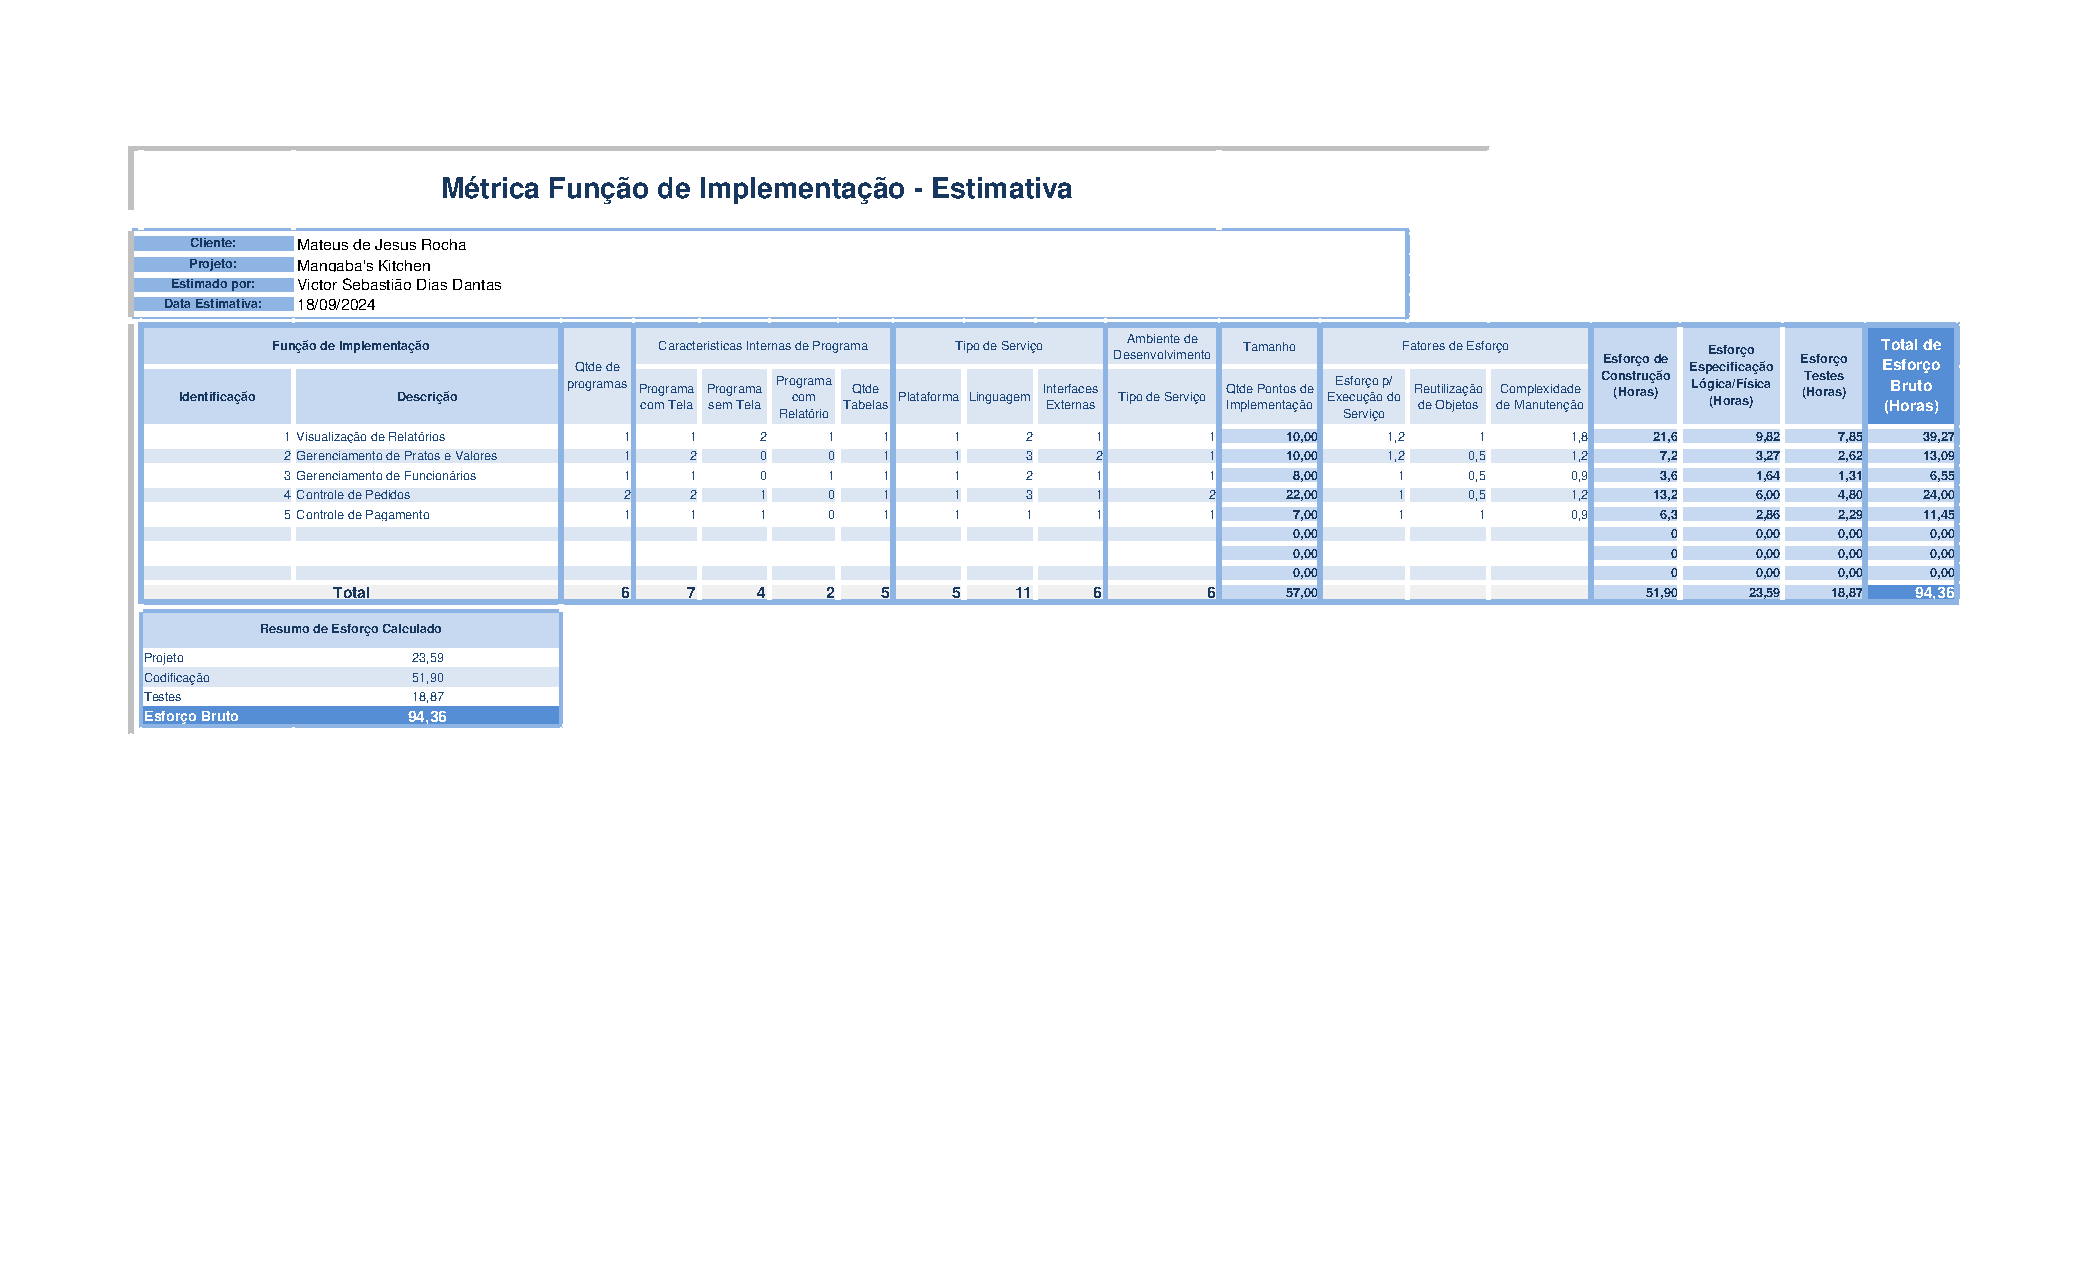
\includepdf[pages=1]{./PDFs/Documento_de_Estimativa.pdf}
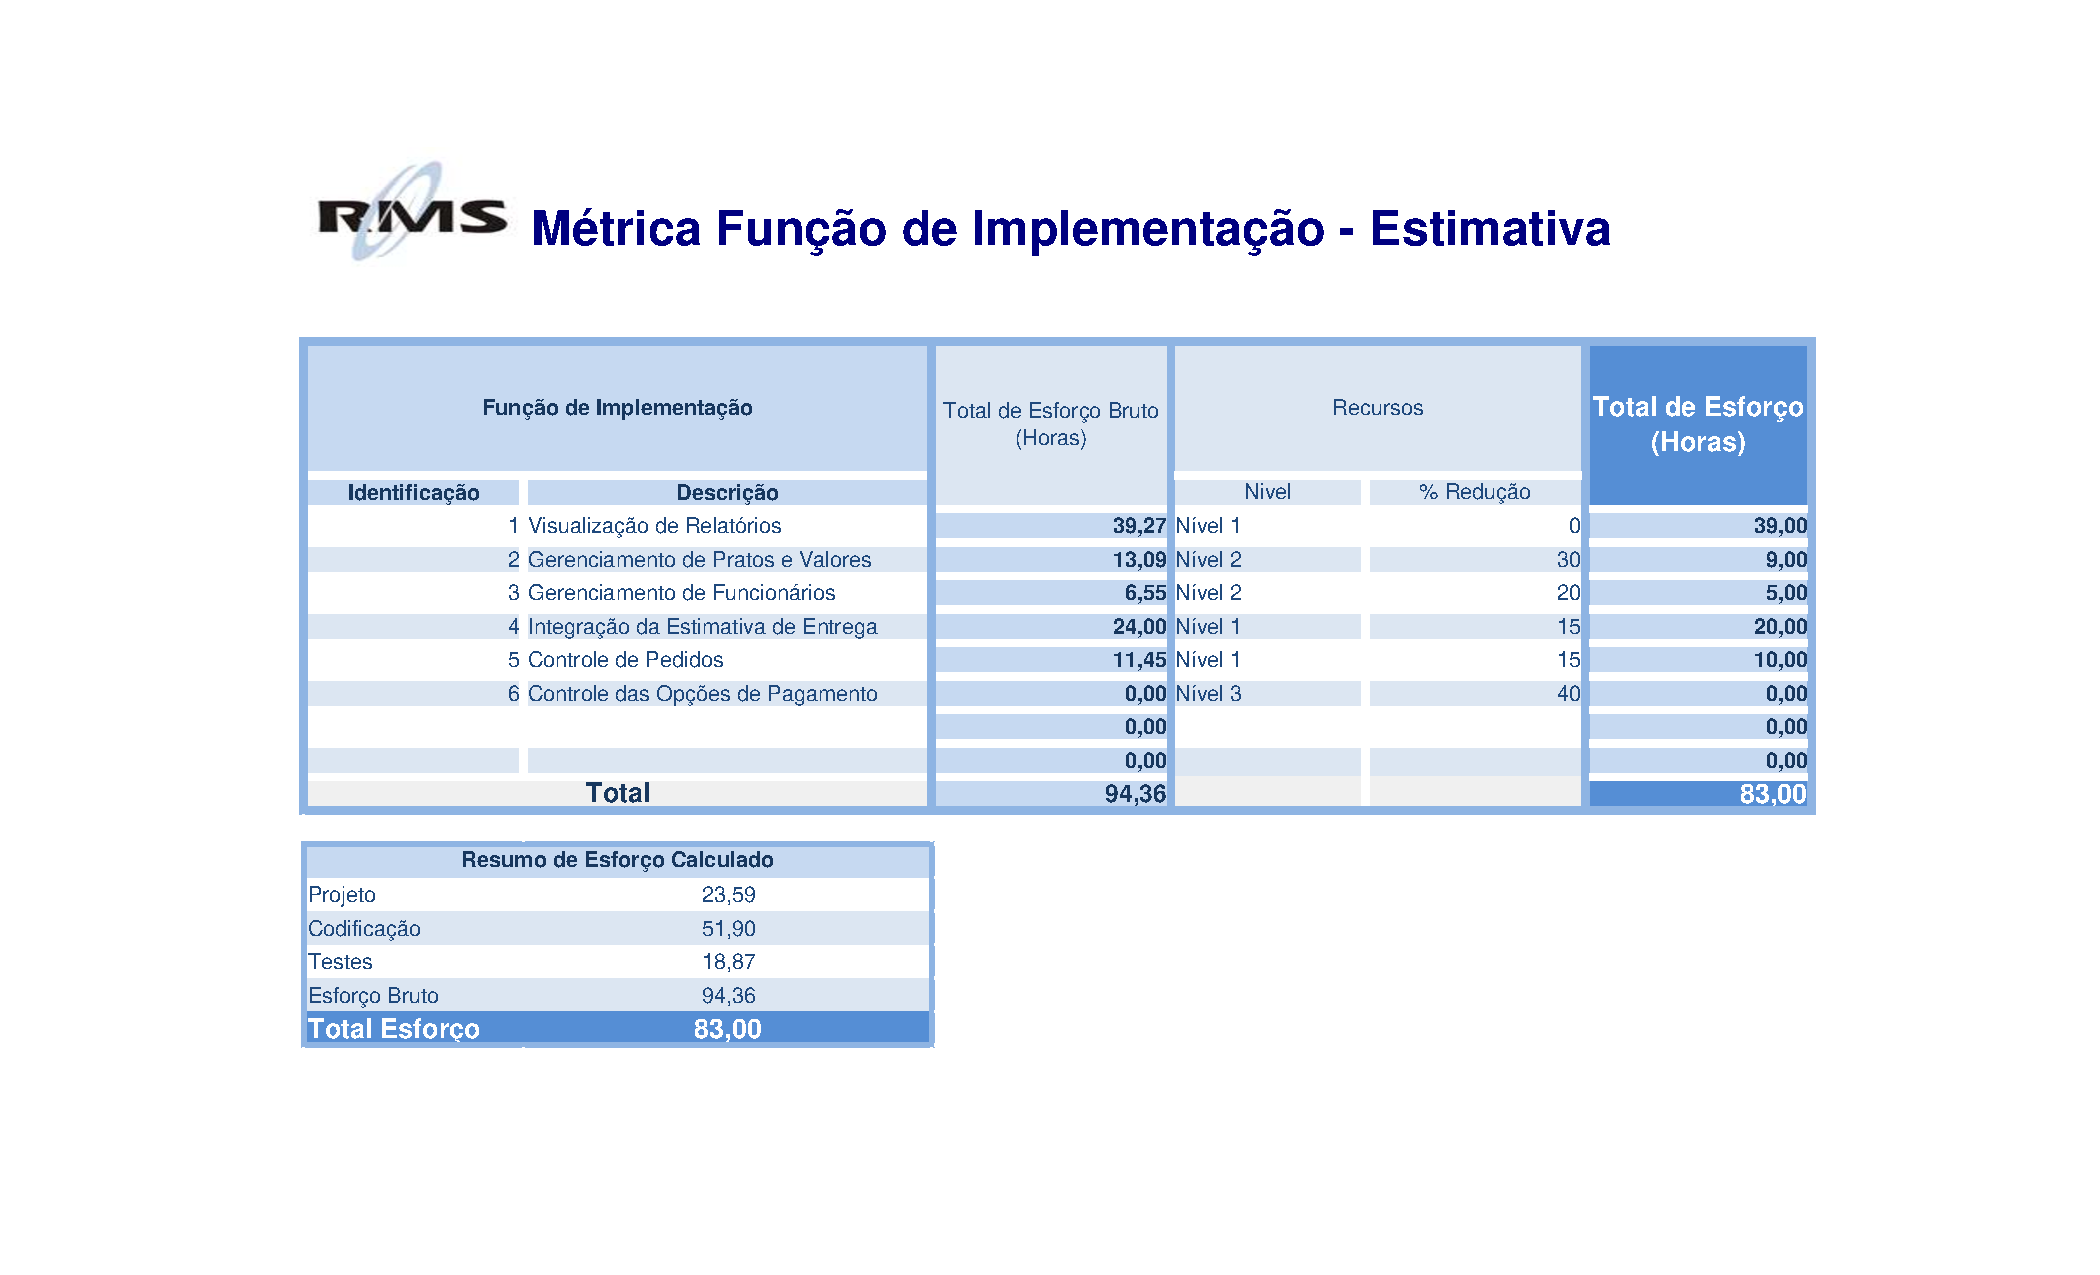
\includepdf[pages=1]{./PDFs/Documento_de_Recursos.pdf}  
    \vspace{12mm}                           
    
    \newpage                                
    \section{Cronograma}                    
        \hspace{4.5mm}
A fase de especificação de requisitos foi agendada para ser concluída até o fim do quarto sprint, com prazo total de um mês, onde será produzido os seguintes documentos: problema, objetivo, documento de requisitos, documento de viabilidade, identidade visual e figma do projeto. Após essa fase, a equipe iniciará a fase de projeto, que está agendada para ser concluída até o terceiro sprint, dia 6 de outubro, com prazo total de duas semanas.
\par
Os sprints, que têm a duração de uma semana, eles começaram no dia 25 de agosto, com reuniões Scrum nos dias úteis, para revisar o progresso e ajustar as estratégias conforme necessário. Os sprints continuam regularmente, com o quarto sprint previsto para terminar no dia 15 de setembro, marcando o fim da fase de levantamento de análise de requisitos do sistema. O cronograma inclui ainda um sprint adicional no dia 18 de setembro para refinamento da apresentação dos artefatos para o cliente.        
    \vspace{12mm}                           
    
    \newpage                                     
    \section{Fundamentação teórica}              
        \hspace{4.5mm}
O cronograma do projeto de informatização do Mangaba's Kitchen foi estruturado utilizando o framework Scrum, que se destaca pela sua abordagem simples, iterativa e incremental. O projeto está dividido em três fases principais: especificação de requisitos, onde será feito o levantamento e análise dos requisitos e refinamento do backlog. Também vai ter a fase de projeto do sistema, onde será definido as funcionalidades e especificações técnicas que serão necessárias para realizar o desenvolvimento do sistema. E por fim a implementação, onde acontecerá o desenvolvimento do sistema. O processo inteiro de desenvolvimento de todos os artefatos de software está dividido em quatro etapas, sendo elas: planejamento, ação, revisão e correção.   
    \vspace{12mm}                                
    
    \newpage                                        
    \section{Termo de aceite do cliente assinado}   
        
\begingroup
\hspace{4.5mm}
\setlength{\parindent}{0pt}


\section*{Termo de Aceite de Contrato de Prestação de Serviços}
\subsection*{Identificação das Partes}

\textbf{Contratante:}\\

\begingroup

    \leftskip 20pt
    \rightskip 20pt
    
    Nome: Mangaba’s Kitchen\\
    Endereço: Salvador-BA\\
    Representante Legal: Mateus de Jesus\\\\

\endgroup

\textbf{Contratada:}\\

\begingroup

    \leftskip 20pt
    \rightskip 20pt
    
    Nome: Mangaba Tech\\
    Endereço: Salvador-BA\\
    Representante Legal: Victor Dantas

\endgroup

\subsection*{Identificação do Programa de Computador (Software)}
Denominação: Sistema de Gerenciamento de Restaurante Mangaba's Kitchen\\\\
Módulo (Objeto): 1 (Uma) cópia do software executável, com licença para uso em tablets para os garçons, em um computador pessoal para o gerente e em uma televisão sensível ao toque para a equipe da cozinha.\\

\subsection*{Requisitos e Funcionalidades}

\leftskip 0pt
\rightskip 0pt
\textbf{I. Objeto.}\\
O presente termo de concordância tem como objetivo validar os requisitos acordados entre as partes para o desenvolvimento do software de gerenciamento de restaurante. O sistema será utilizado para automação de vendas, controle de estoque, gestão de pedidos e geração de relatórios financeiros.\\

\begingroup

    \leftskip 20pt
    \rightskip 20pt
    
    § 1º – A Contratante concorda que o software inclui funcionalidades para gerenciamento de pedidos, como estimativa de tempo de preparo, atualização dos status dos pedidos e consulta ao histórico de pedidos.\\\\
    § 2º – A Contratante está de acordo com as funcionalidades abordadas no modelo protótipo feito no Figma, e está de acordo com visual do programa.\\\\
    § 3º – A Contratada garante a protação de dados da Contratante, conforme a Lei Geral de Proteção de Dados - Lei n° 13709/2018 - LGPD.\\\\
    § 4º – A Contratada fornecerá suporte técnico e correção de erros pelo período de 6 (seis) meses a partir da data de implementação do sistema.\\\\
    § 5º – Caso a Contratante solicite versões adicionais ou melhorias, tais solicitações serão objeto de novos acordos ou aditivos contratuais.\\\\
    
\endgroup

\textbf{II. Preços e Condições de Pagamento.}\\
Os preços estão descritos no preâmbulo deste termo e seguem as seguintes condições:
O valor total será pago em parcela única no ato de implementação do sistema, conforme acordado previamente.\\\\


\textbf{III. Instalação, Implantação e Treinamento.}\\
Para a instalação do sistema, a Contratante deverá disponibilizar equipamentos com configuração mínima conforme descrito previamente. Manuais detalhados com todas as instruções necessárias serão fornecidos para garantir a instalação e operação correta do software.

Se necessário, a Contratada poderá realizar o serviço de instalação e treinamento mediante acordo, sem custo adicional para clientes da cidade de Salvador. Para clientes de outras localidades, os custos de viagem e hospedagem serão negociados entre as partes.\\\\


\textbf{IV. Vigência e Atualizações.}\\
Este termo entra em vigor na data de sua assinatura, e o uso do software será válido por prazo indeterminado, incluindo versões futuras adquiridas pela Contratante.\\\\


\textbf{V. Direito de Propriedade e Uso.}\\
O software é propriedade da Contratada, que concede à Contratante o direito de uso conforme os requisitos estabelecidos neste termo. É vedado à Contratante realizar cópias, sublicenciar ou modificar o sistema sem a devida autorização.\\

\begingroup

    \leftskip 20pt
    \rightskip 20pt
    
    § ÚNICO – A Contratante é responsável por manter o sigilo sobre o sistema e seu uso, conforme previsto na legislação vigente.\\\\

\endgroup

\textbf{VI. Garantia Limitada.}\\
A Contratada garante que o software funcionará conforme as especificações por um período de 180 dias, oferecendo substituição de mídias de instalação defeituosas dentro de 60 dias após a entrega.\\\\


\textbf{VII. Outras Condições.}\\
A Contratante deverá seguir as recomendações técnicas fornecidas para garantir o pleno funcionamento do sistema. Caso surjam dúvidas que possam ser sanadas pelo manual, a Contratada não será obrigada a prestar suporte adicional.\\\\

Por estarem de acordo com os requisitos descritos, as partes assinam este termo de concordância em duas vias de igual teor.\\\\

Salvador, Bahia, 17 de Setembro de 2024\\\\

\endgroup

\begin{center}
    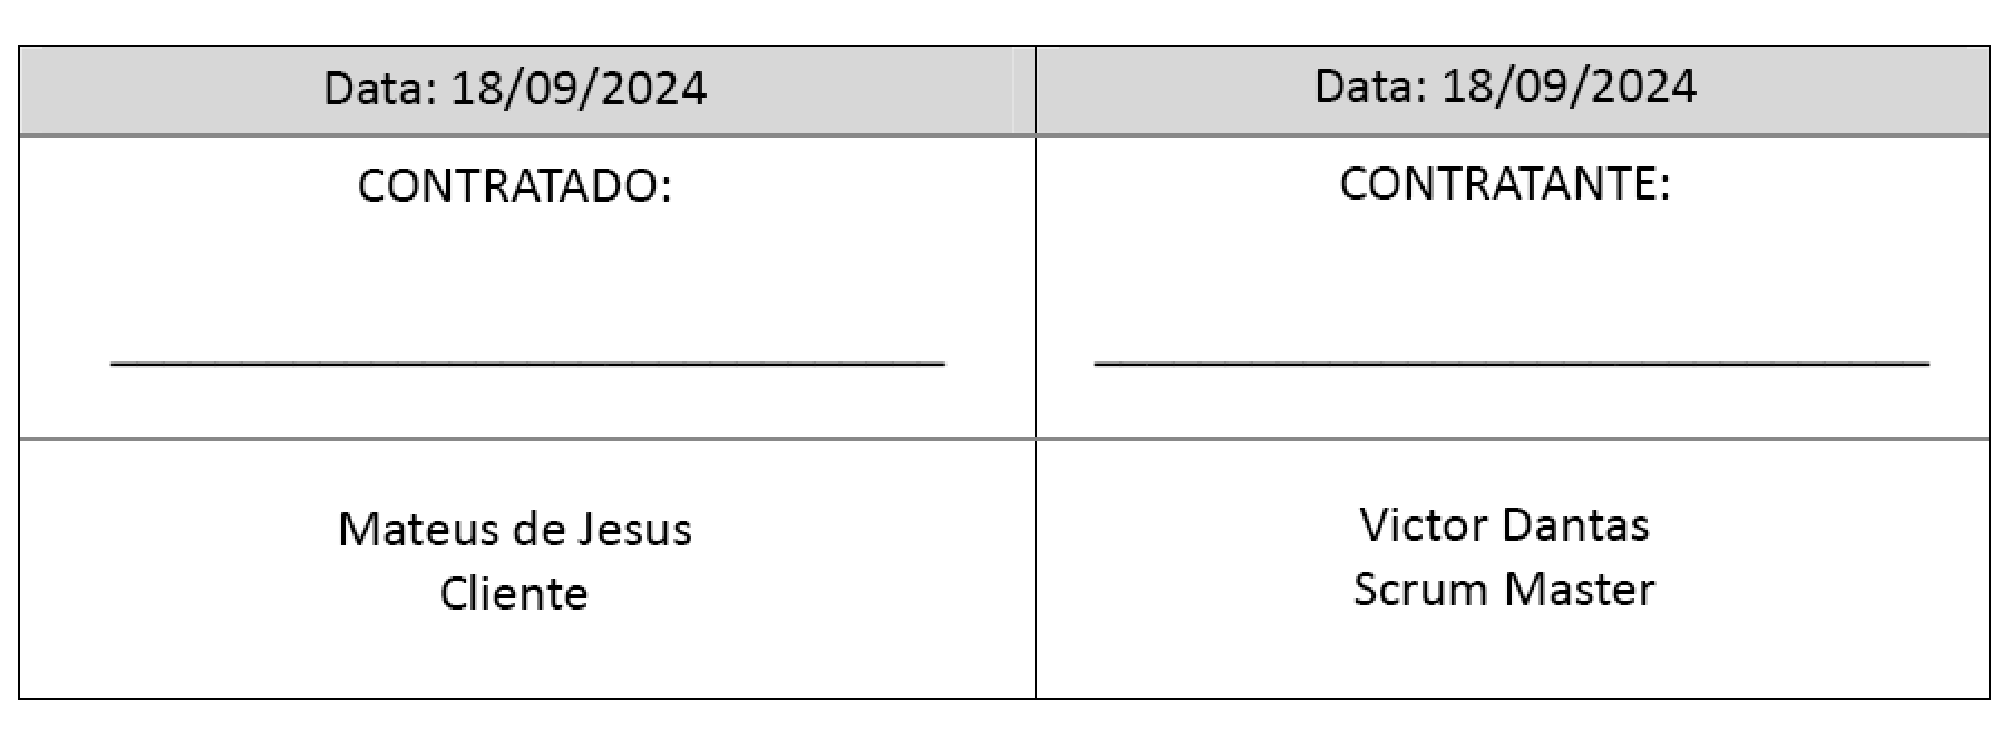
\includegraphics[width=1\textwidth]{PDFs/Assinatura.pdf} 
\end{center}             
    \vspace{12mm}                                   
    
    \newpage                                
    \section{Conclusão}                     
        \hspace{4.5mm}
Portanto, a proposta de informatização do Mangaba Kitchen visa transformar como o restaurante gerencia suas operações diárias, abordando diretamente as dificuldades enfrentadas na coordenação entre a equipe e no controle de pedidos. A introdução de um sistema integrado que inclui interfaces específicas para gerentes, garçons e cozinheiros permitirá uma gestão mais eficiente dos pedidos, um controle aprimorado das estimativas de entrega e uma comunicação mais fluida entre as áreas. Com funcionalidades como cadastro e gerenciamento de funcionários, acompanhamento de pedidos e geração de relatórios financeiros, o sistema visa não apenas otimizar a operação interna, mas também melhorar a experiência do cliente, reduzindo atrasos e erros que impactam a satisfação dos consumidores.
\par
A viabilidade econômica e técnica do projeto está bem sustentada pela clareza dos requisitos e pela experiência da equipe de desenvolvimento, que possui conhecimento profundo das ferramentas e tecnologias necessárias. O cronograma estruturado utilizando o framework Scrum, com fases definidas e sprints regulares, assegura que cada etapa do desenvolvimento será cuidadosamente monitorada e ajustada conforme necessário. A combinação de uma estratégia bem planejada, a escolha adequada de dispositivos e a abordagem iterativa garantem que o sistema será implementado eficientemente, alinhando-se às necessidades operacionais do Mangaba Kitchen e promovendo uma operação mais ágil e eficiente.         
    
    % Formatação da bibliografia
    % bibliographystyle{plain}
    % \newpage
    % \bibliography{referencias} % Assume que você tem um arquivo referencias.bib
    
\end{document}
